\documentclass[12pt,a4paper]{article}
\usepackage[utf8]{inputenc}
\usepackage{amsmath}
\usepackage{amsfonts}
\usepackage{amssymb}
\usepackage[top=3cm, bottom=2cm, left=3cm, right=2cm]{geometry} % geometria da pagina
\usepackage{natbib} 			% Fazer referencias bibliograficas

 %comandos criados pelo fabbri
\newcommand{\etc}{{\it etc}}
\newcommand{\ie}{{\it i.e.}}
\newcommand{\eg}{{\it e.g.}}
\newcommand{\wrt}{{\it w.r.t. }}
\newcommand{\etal}{{\it et.~al.}}
\newcommand{\intinf}{\int_{-\infty}^{\infty}}
\newcommand{\grad}{\nabla}
\newcommand{\slant}{\sigma}
\newcommand{\R}{\mathbb{R}} % the reals
\newcommand{\trace}{\text{trace}\,}
%\newcommand{\det}{\text{det}}

% skew-symmetric arrangement
\newcommand{\skewm}[1]{{#1}_\times}

\renewcommand{\vec}[1]{\mathbf{#1}}

\newcommand{\lbar}{\overline}

\newcommand{\id}{\text{\emph{I}}}
\newcommand{\dof}{\textsc{dof}}
\newcommand{\ransac}{\textsc{ransac}}
\newcommand{\sift}{\textsc{sift}}
\newcommand{\klt}{\textsc{klt}}
\newcommand{\svd}{\textsc{svd}}
\newcommand{\sfm}{\textsc{sfm}}
\newcommand{\rot}{\mathcal{R}}
\newcommand{\brot}{\overline{\mathcal{R}}}
\newcommand{\Gama}{\boldsymbol{\Gamma}}
\newcommand{\gama}{\boldsymbol{\gamma}}
\newcommand{\gamad}{\dot{\gama}}
\newcommand{\bsigma}{\boldsymbol{\sigma}}
\newcommand{\T}{\boldsymbol{T}}
\newcommand{\N}{\mathbf{N}}
\newcommand{\NSurface}{\mathbf{N}}
\newcommand{\Nlocal}{\overline{\N}} % normal in local coordinates
\newcommand{\balpha}{\boldsymbol{\alpha}}
\newcommand{\tDt}{t+\Delta t}
\newcommand{\bpsi}{\boldsymbol{\boldsymbol{\psi}}}
\newcommand{\bp}{\mathbf p}
\newcommand{\deldt}[1]{\frac{\partial#1}{\partial t}}
\newcommand{\ddt}[1]{\frac{d #1}{dt}}
\newcommand{\delds}[1]{\frac{\partial#1}{\partial s}}
\newcommand{\mybar}[1]{\overline{#1}}
\newcommand{\norm}[1]{\|#1\|}
\newcommand{\I}{\mathbf{I}}
\newcommand{\brho}{\boldsymbol{\rho}}
\newcommand{\lightrgb}{\boldsymbol{l}}
\newcommand{\B}{\boldsymbol{B}}
\renewcommand{\t}{\boldsymbol{t}}
\newcommand{\n}{\boldsymbol{n}}
\renewcommand{\b}{\boldsymbol{b}}
\newcommand{\e}{\boldsymbol{e}}
\newcommand{\f}{\boldsymbol{F}}
\newcommand{\hf}{\boldsymbol{\hat{f}}}
\newcommand{\g}{\boldsymbol{g}}
\newcommand{\G}{\boldsymbol{G}}
\newcommand{\bc}{\boldsymbol{c}}
\newcommand{\Curve}{\boldsymbol{\mathcal{C}}}
%\newcommand{\X}{\boldsymbol{X}}
%\newcommand{\x}{\boldsymbol{x}}
\newcommand{\X}{\mathbf{X}}
\newcommand{\x}{\mathbf{x}}
\newcommand{\xx}{\mathcal{X}}  % used in Giblin's notes
\newcommand{\tilx}{\tilde x}
\newcommand{\tily}{\tilde y}
\newcommand{\tilgama}{\tilde \gama}
\newcommand{\ugama}{\hat{\gama}} %unit gama
\newcommand{\br}{\bar r}
\newcommand{\Kc}{\mathbf K_c}
\newcommand{\lepi}{\mathbf r}
\newcommand{\itan}{\tan^{-1}}
\newcommand{\uu}{\xi}
\newcommand{\buu}{\bar \uu}
\newcommand{\bvv}{\bar \vv}
\newcommand{\vv}{\eta}
\newcommand{\VV}{\mathbf{V}} % translational velocity
\newcommand{\VVspeed}{V} % translational velocity
\newcommand{\field}{\boldsymbol\chi}
\newcommand{\ufield}{\hat{\boldsymbol{\chi}}}
\newcommand{\fieldc}{\chi} % field component
\newcommand{\transl}{\mathcal{T}} % field component
\newcommand{\btransl}{\overline{\mathcal{T}}} % field component
\newcommand{\albedo}{\alpha}
\newcommand{\depth}{\rho}      % depth as z
\newcommand{\ddepth}{\dot{\rho}}      % depth as z
\renewcommand{\l}{\lambda} % used in problem2-thoughts-giblin
\newcommand{\udepth}{{\hat{\rho}}} % depth along ray
\newcommand{\ttransl}{\T} % translation tangent
\newcommand{\surface}{\mathcal{M}} % surface/manifold
\newcommand{\surf}{\mathcal{M}} % surface/manifold short
\newcommand{\jacm}{\mathtt{J}} % Jacobian matrix
\newcommand{\xbar}{\bar x}
\newcommand{\ybar}{\bar y}
\newcommand{\zbar}{\bar z}

\newcommand{\bdelta}{\boldsymbol \delta}
%\newcommand{\X}{\boldsymbol{X}}
%\newcommand{\x}{\boldsymbol{x}}
%\newcommand{\X}{\mathbf{X}}
%\newcommand{\x}{\mathbf{x}}
\newcommand{\boldu}{\mathbf{u}}
\newcommand{\boldv}{\mathbf{v}}
\newcommand{\boldw}{\mathbf{w}}
\newcommand{\tgtveloc}{\tilde\alpha} % real tangential velocity



\begin{document}

\newpage
\pagestyle{headings}
\section{Introdução}
A Visão Computacional é uma área de pesquisa que se ocupa em utilizar imagens em 2D de um cenário, obtidas de uma ou mais câmeras digitais para produzir uma construção virtual em 3D, ou extrair qualquer outro tipo de informação útil como o cruzamento de informações entre imagens. A captação da geometria 3D de um cenário a partir de imagens produzidas por câmeras, analisando a disparidade entre elementos correspondentes nessas imagens, é chamada de visão {\it estereoscópica}, da qual a visão computacional se utiliza para desenvolver modelos adequados à descrição geométrica tanto da cena 3D em questão como das câmeras que fazem a projeção da cena na imagem 2D.  

\begin{figure}[!htb]
\centering
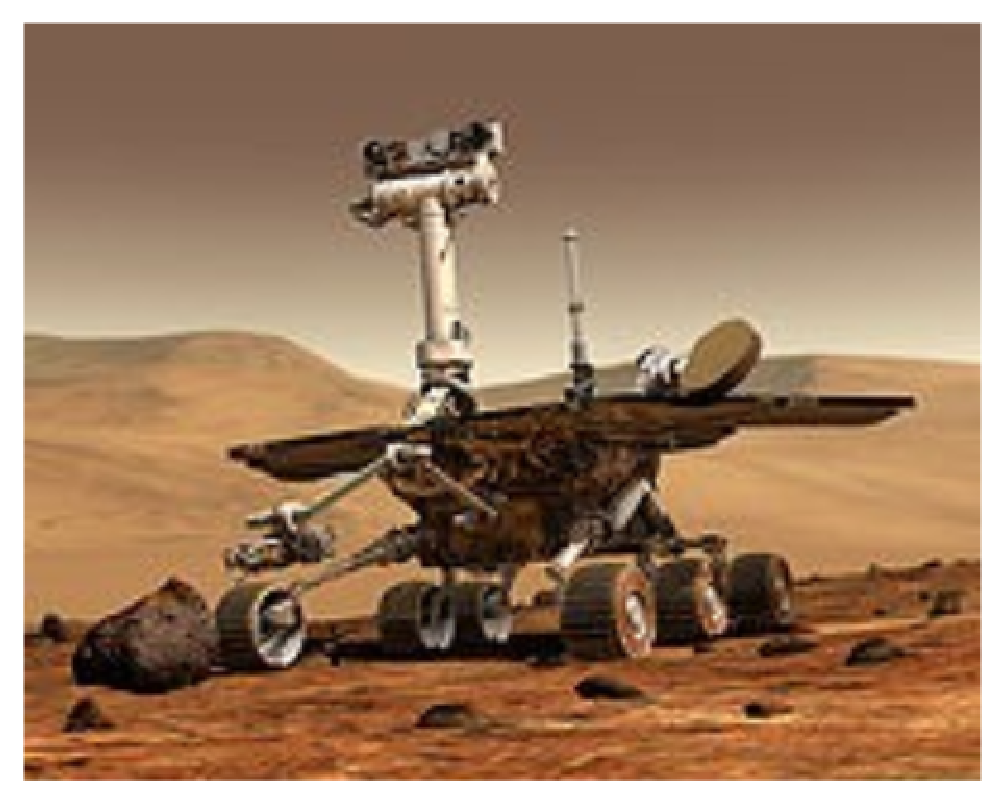
\includegraphics[scale=.5]{mars-rover}
\caption{{\it O maior passo no uso de visão computacional em pesquisas interplanetárias foi dado na missao NASA/JPL Mars Exploration Rover (MER).}}
\label{fig.mars-rover}
\end{figure}

A geometria projetiva é a principal teoria matemática usada em visão computacional tridimensional. Com a introdução de algumas definições e conceitos, a geometria projetiva pode ser estudada em termos de álgebra linear, onde tal abordagem traz alguns benefícios de modelagem e é amplamente utilizada por pesquisadores dessa área, mas também possui algumas limitações. Em pesquisas mais recentes, verificou-se a eficácia do uso de técnicas de geometria algébrica em resoluções de sistemas de equações polinomiais, oriundos de problemas de visão computacional 3D. Mais recentemente ainda, \citep{tese-fabbri} introduziram uma abordagem em termos de geometria diferencial, onde é possível aplicar o cálculo diferencial trabalhando diretamente com as equações algébricas. Essa abordagem permite um maior poder de modelagem matemática e computacional do espaço tridimensional através das imagens.


\subsection*{Motivação}
As motivações para a pesquisa estão ligadas às suas aplicações em diversas áreas. A extração de informação da geometria 3D de um ambiente pode, por exemplo, ser utilizada na determinação da orientação e posição de veículos autônomos, para que os mesmos identifiquem a trajetória para os seus objetivos considerando a possibilidade de obstáculos. Um exemplo famoso, segundo \citep{mars-rover}, é a aplicação em pesquisas interplanetárias onde foram usados algoritmos de visão computacional em veículos de exploração de Marte (Mars Exploration Rover - MER, em inglês), observado na figura \ref{fig.mars-rover}.


Uma aplicação mais recente foi a reconstrução virtual de objetos, estátuas ou monumentos de valor histórico e cultural que tenham sido destruídos pela ação do tempo ou do homem (possivelmente em guerras), através da aquisição de imagens em acervos ou na internet. Um exemplo é o Museu de Mosul {\footnote{Outros exemplos podem ser encontrados em http://www.projectmosul.org/}}, no Iraque, atacado pelo 
Estado Islâmico em 2015, que teve algumas de suas obras reconstruídas como podemos visualizar na figura \ref{fig.mossul}.

\begin{figure}[!htb]
\centering
\subfloat{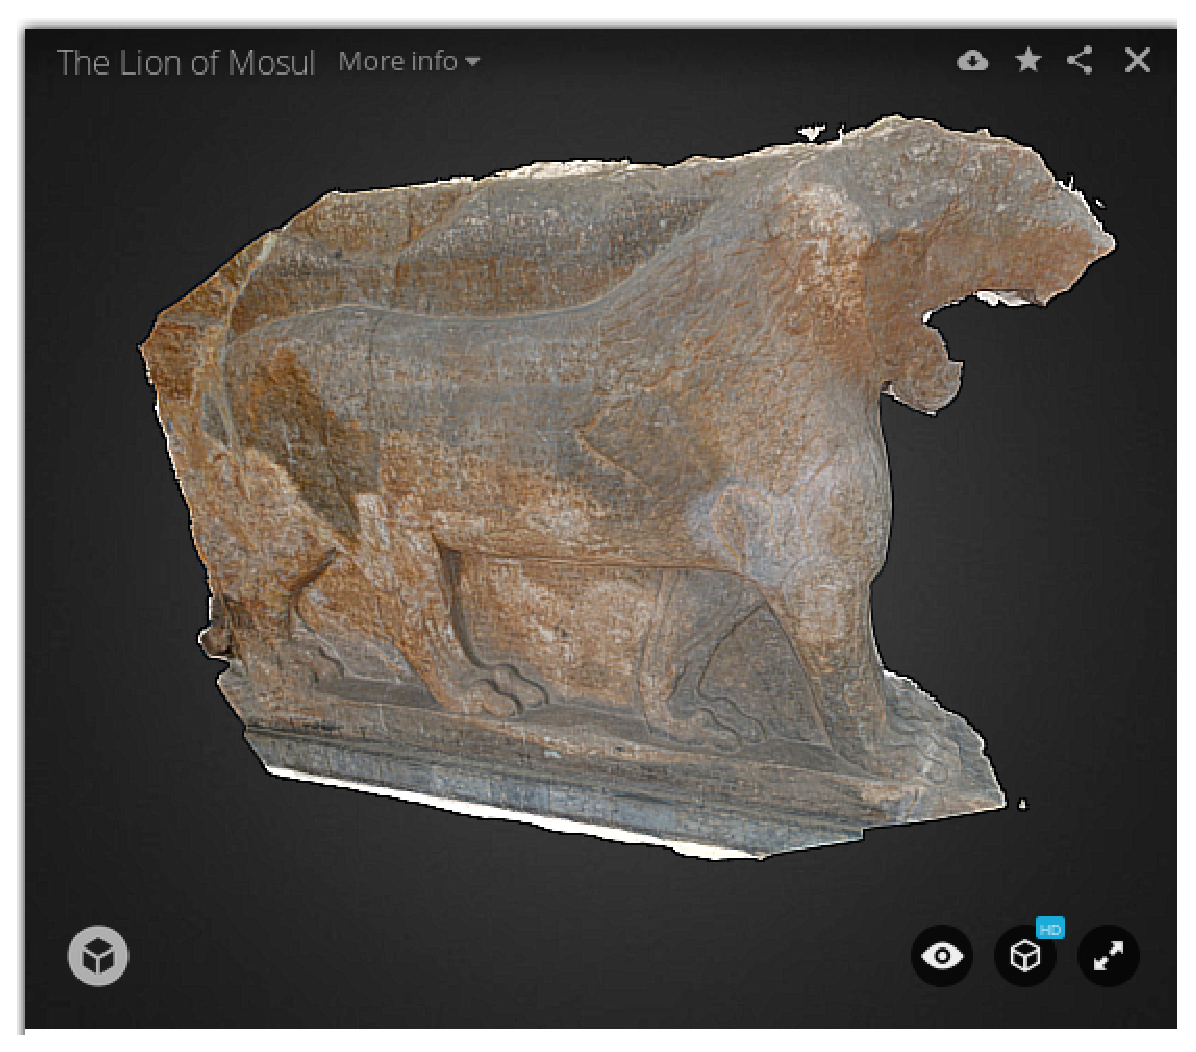
\includegraphics[scale=.385]{leao-mosul}}
\quad
\subfloat{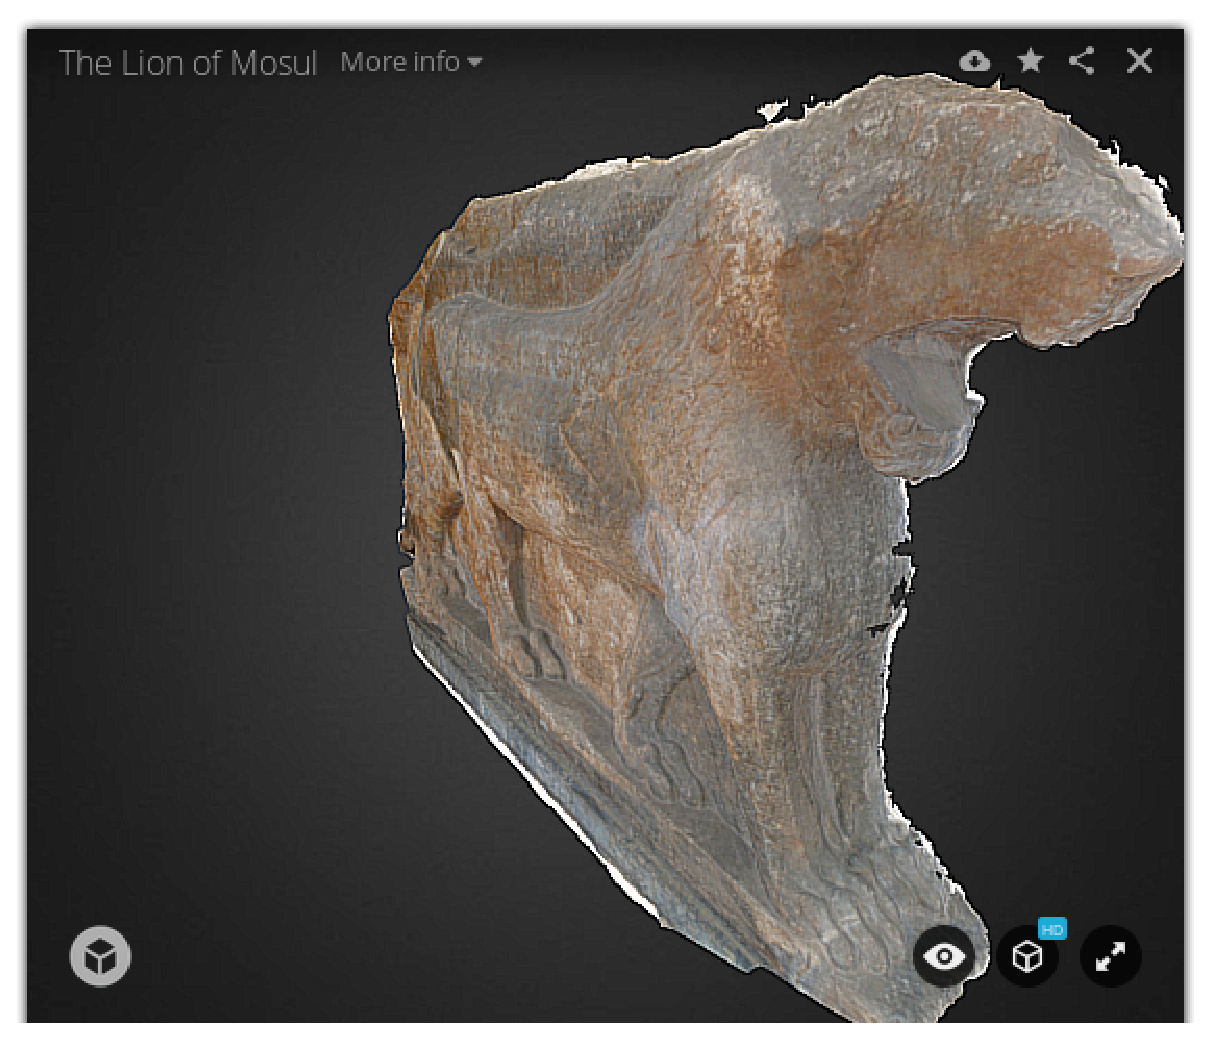
\includegraphics[scale=.385]{lion-mosul-2}}
\caption{{\it A reconstrução do Leão de Mosul, um dos artefatos destruídos por extremistas religiosos em 2015 no Iraque.}}
\label{fig.mossul}
\end{figure}

As aplicações de visão computacional são bastante variadas, com pesquisas em outras áreas como astronomia, medicina e química. Para se ter uma ideia, \citep{ballard-82} já apresentavam imagens e tabelas com resumos de aplicações em oito áreas diferentes no início dos anos 1980.  

Novos avanços em reconstrução 3D vêm sendo realizados constantemente como observamos em \citep{fabbri-drawing}, que apresentam uma abordagem para a reconstrução de um esboço 3D (3D drawing em inglês) de uma cena. Isto é, um conjunto de fragmentos de curvas em 3D interligadas de forma que preserve suas relações espaciais, capturadas em forma de gráficos a partir de um grande conjunto de dados multifocal. A ideia base é aprimorar uma abordagem anterior (3D curve sketch) divulgada pelos mesmos autores, \citep{fabbri-sketch}, conforme exemplo visualizado na figura \ref{fig.drawing}.
\begin{figure}[!htb]
\centering
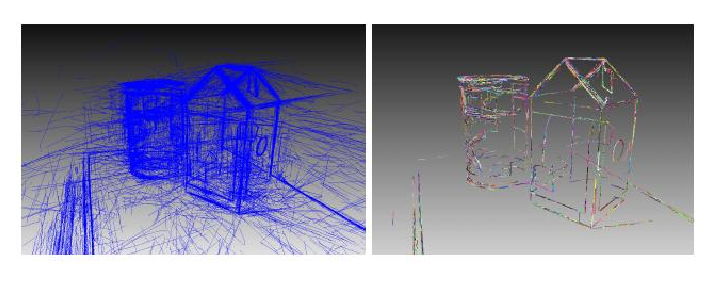
\includegraphics[scale=1.1]{3D-drawing}
\caption{{\it Uma comparação visual: à esquerda os resultados com o 3D curve sketch e à direita os resultados após o aprimoramento com 3D drawing. Repare na redução significante de outliers sem prejuízo do esboço da superfície.}}
\label{fig.drawing}
\end{figure}

A maioria dos métodos de reconstrução não utilizam geometria diferencial de curvas, mas se baseiam em correlacionar pontos de interesse através das imagens e produzem uma desorganizada nuvem de pontos em 3D, figura \ref{fig.medusa}. Tais métodos obtêm sucesso em ambientes controlados, com cenas em larga escala e imagens ricas em textura, mas não podem ser aplicados em configurações gerais. Não podem reconstruir superfícies suaves e homogêneas nem suas fronteiras devido a esparsidade de pontos de interesse, como também não podem reconstruir regiões que se alteram drasticamente com a mudança de luz ambiente. Exemplos de imagens sujeitas a essas limitações são dados na figura \ref{fig.carro-objeto-curvo}.
\begin{figure}[!htb]
\centering
\subfloat{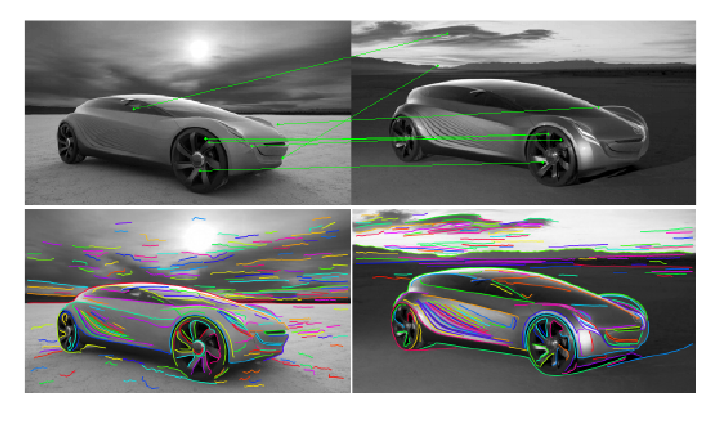
\includegraphics[scale=.76]{carro}}
\quad
\subfloat{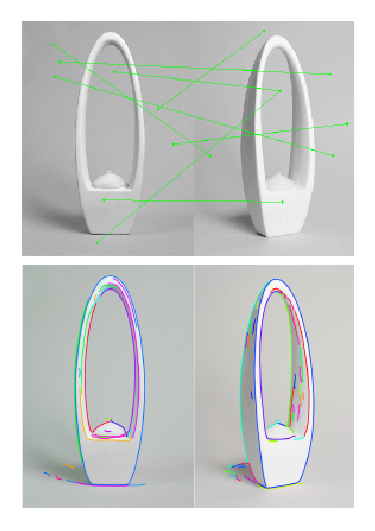
\includegraphics[scale=.6]{objeto-curvo}}
\caption{{\it Exemplos de objetos que não podem ser reconstruídos através da abordagem tradicional usando pontos de interesse e a geometria epipolar.}}
\label{fig.carro-objeto-curvo}
\end{figure}  
Daí são utilizadas outras técnicas de melhoramento dos resultados, como a Interpolação de Pontos e Texturização, mas que não fornecem um resultado plenamente satisfatório. Podemos ver as fases desse processo em um exemplo no conjunto de imagens na figura\ref{fig.medusa}.

Portanto, ainda é necessário que se continuem as pesquisas em visão computacional, e o presente trabalho tem a finalidade de, primeiramente, detalhar as abordagens de artigos recentes na busca de novas combinações de ferramentas matemáticas que possam melhorar as atuais abordagens e atenuar o esforço computacional. Segundo, a verificação dos benefícios obtidos com o uso da geometria trifocal em transferência de pontos e reconstrução 3D em comparação com a geometria epipolar (mais usada atualmente), tudo com o objetivo de auxiliar na construção de uma nova abordagem usando geometria diferencial multifocal em condições realísticas.

\begin{figure}[!htb]
\centering
\subfloat{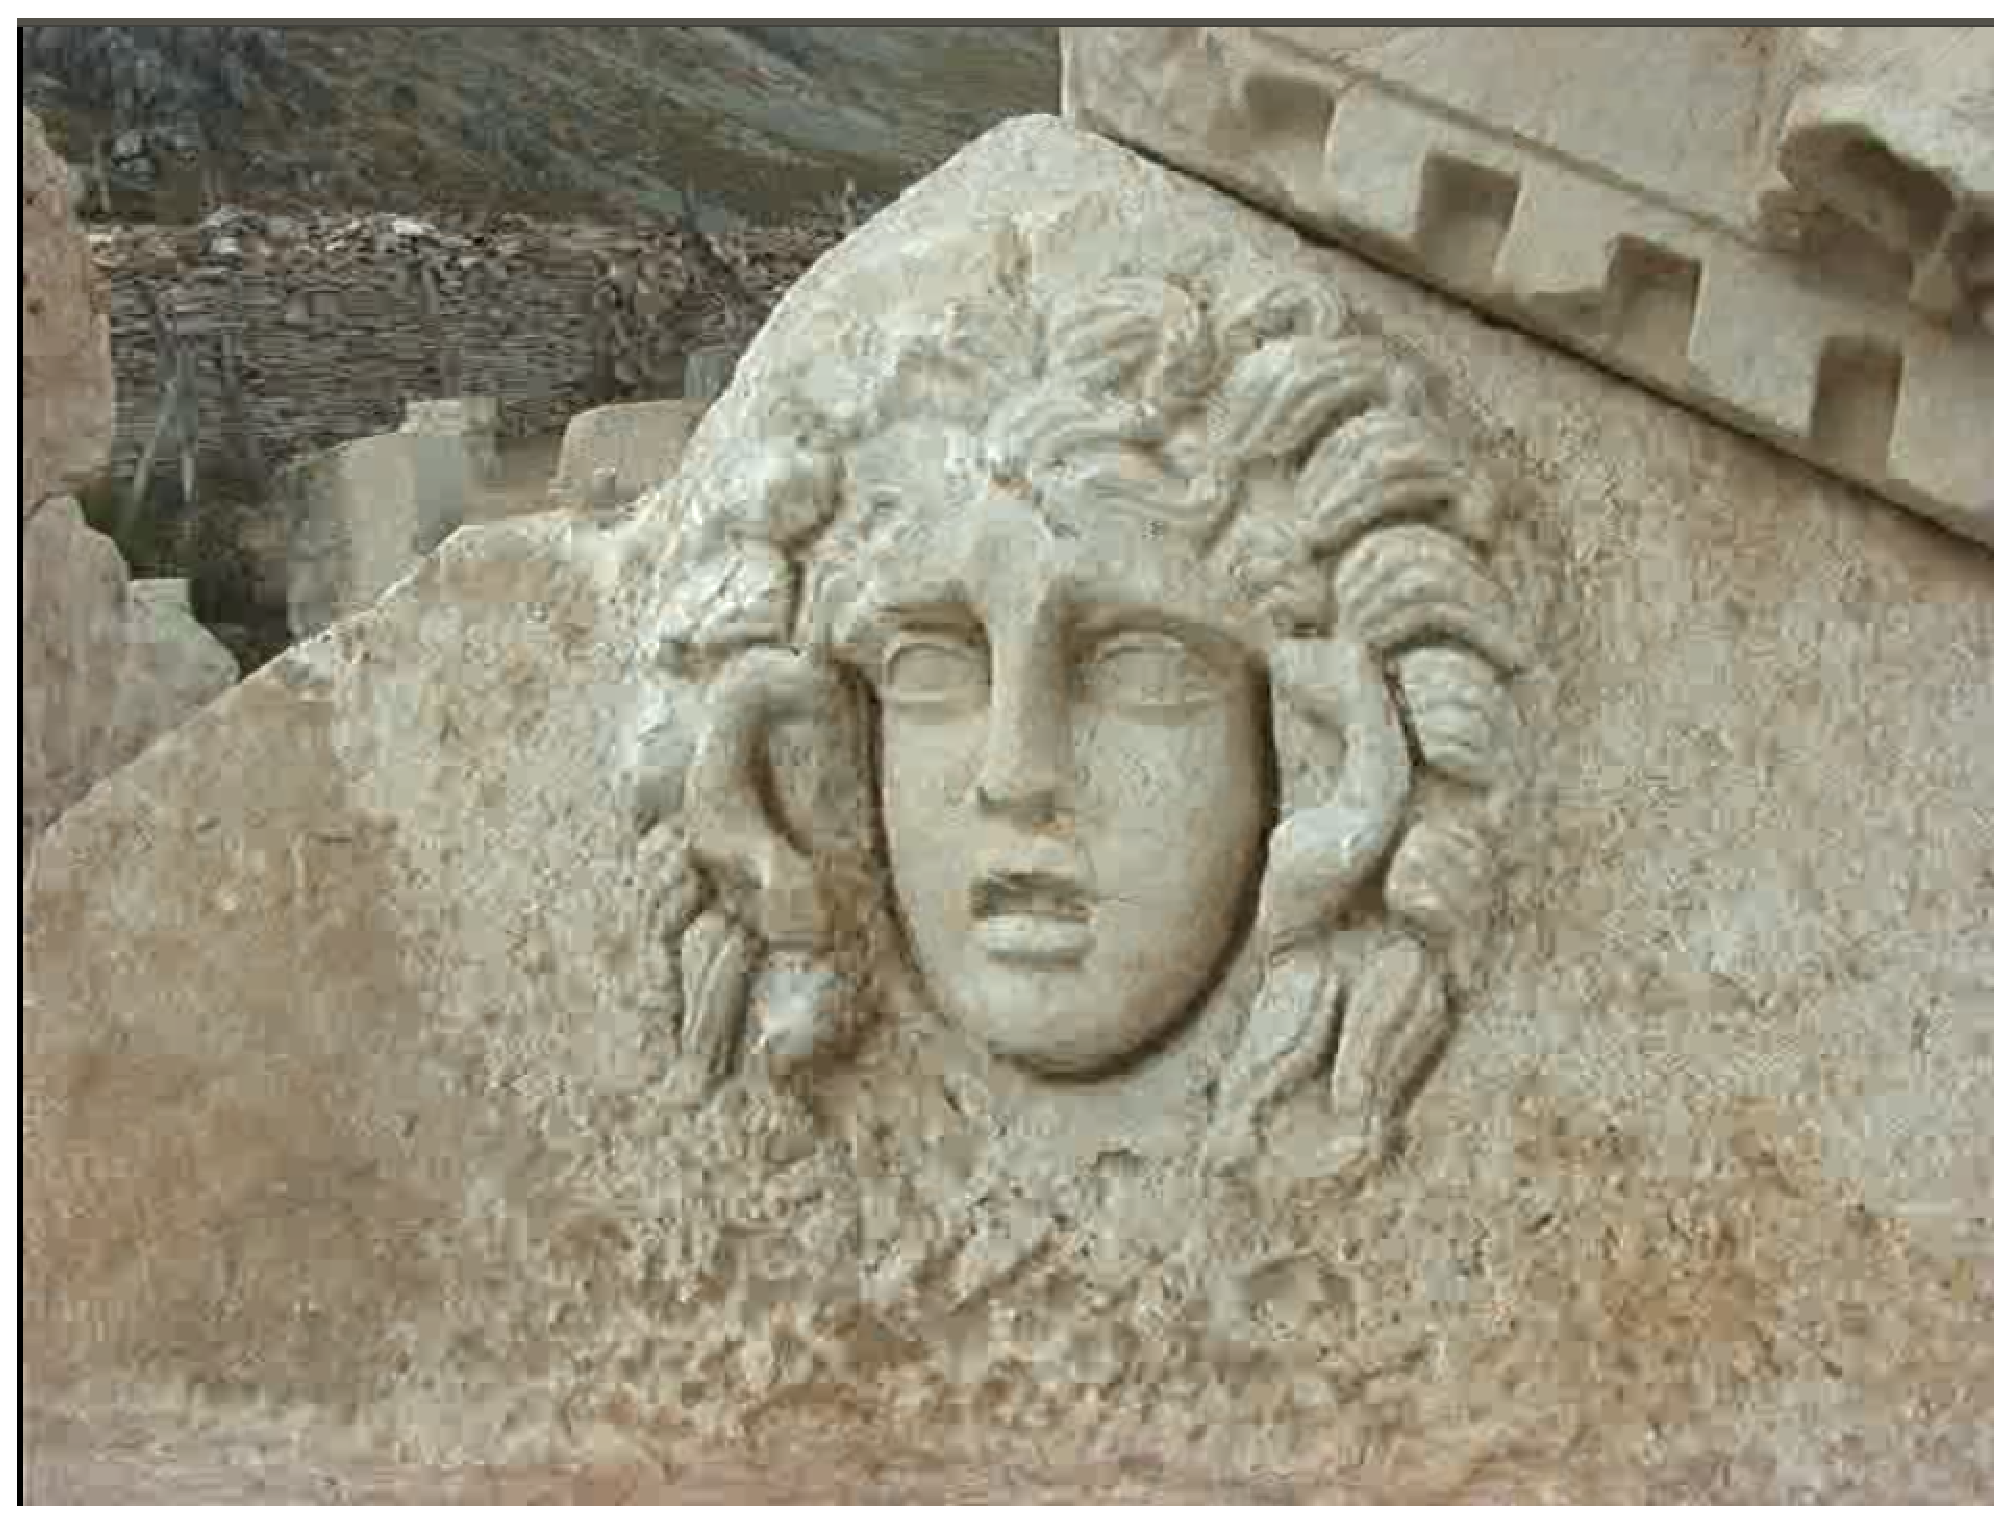
\includegraphics[scale=.2]{medusa1}}
\quad
\subfloat{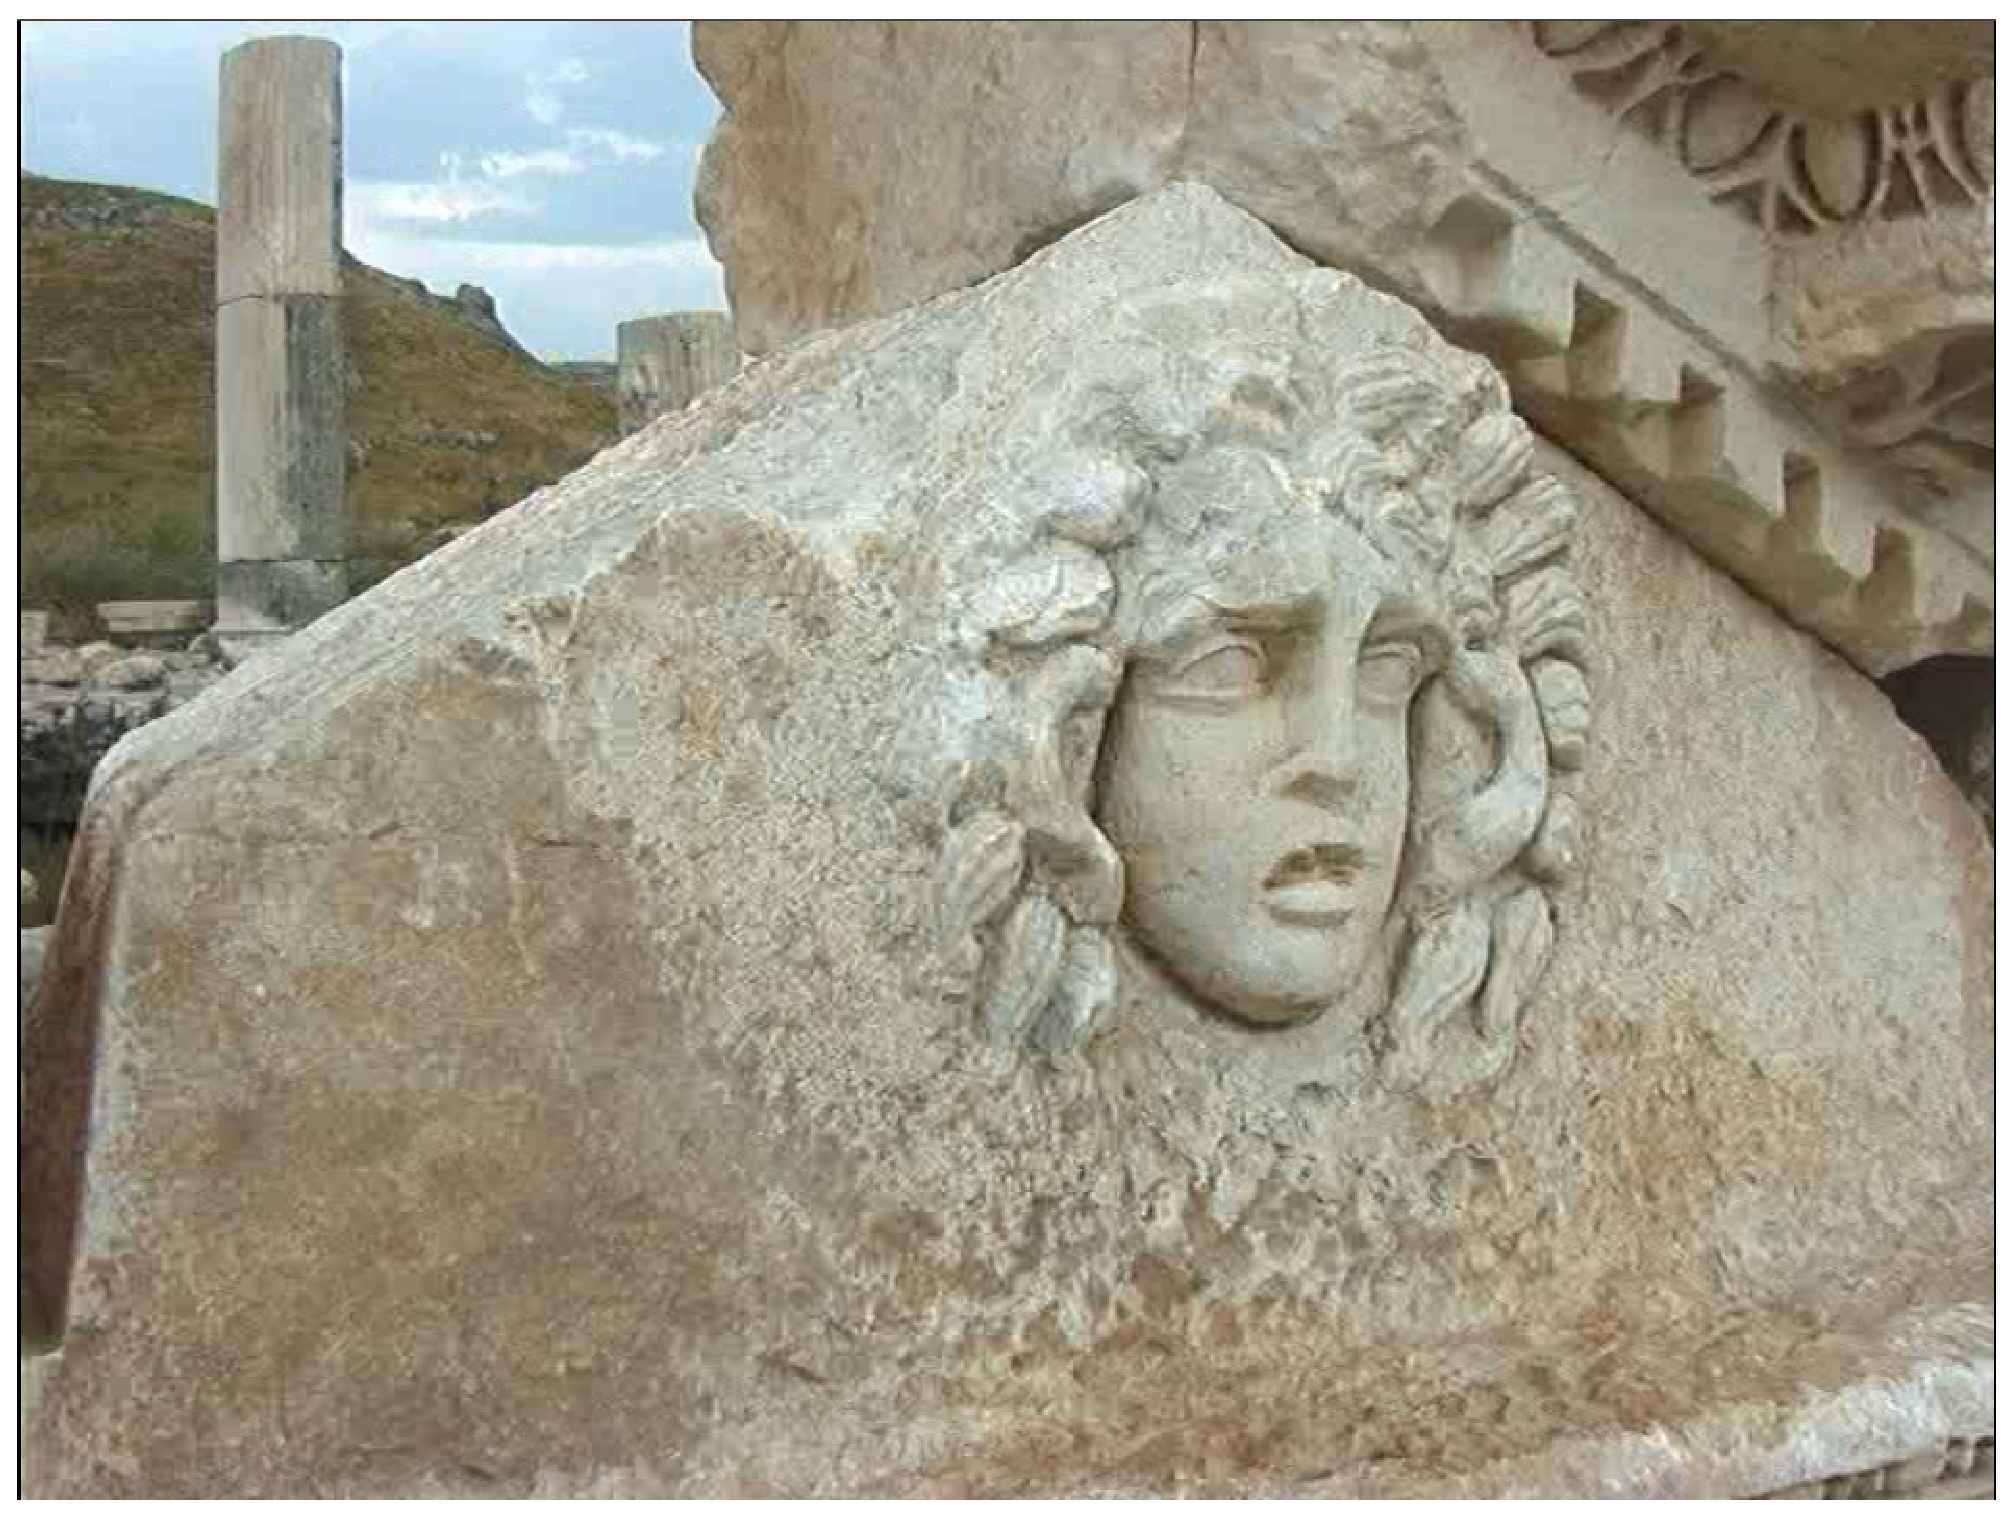
\includegraphics[scale=.2]{medusa2}}
\\
\subfloat{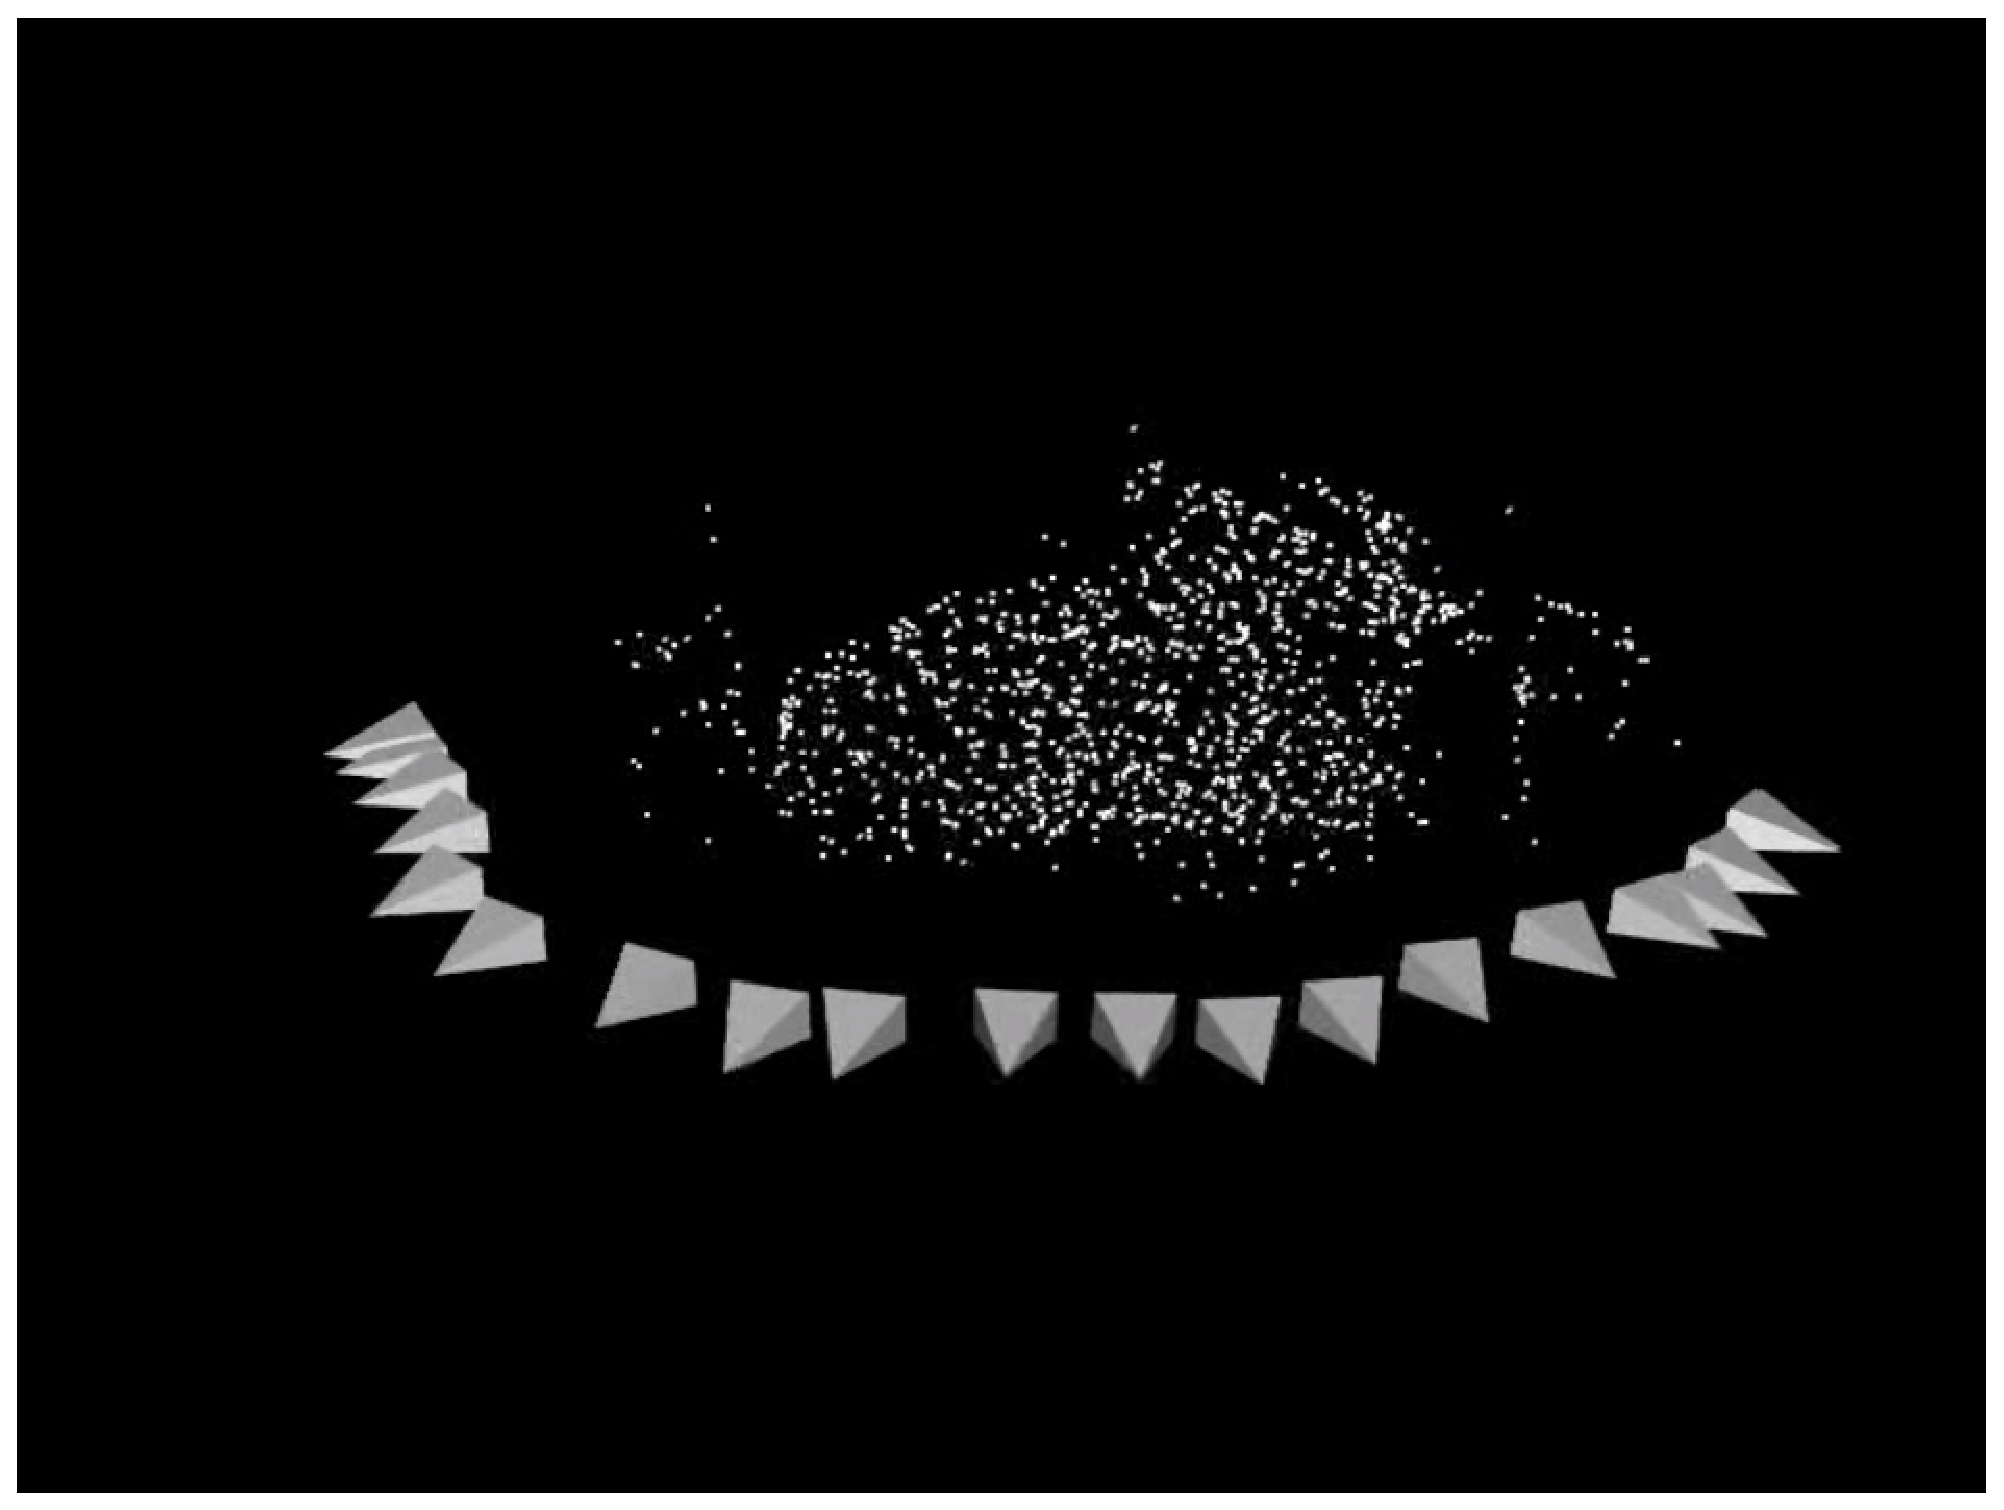
\includegraphics[scale=.2]{nuvem1}}
\quad
\subfloat{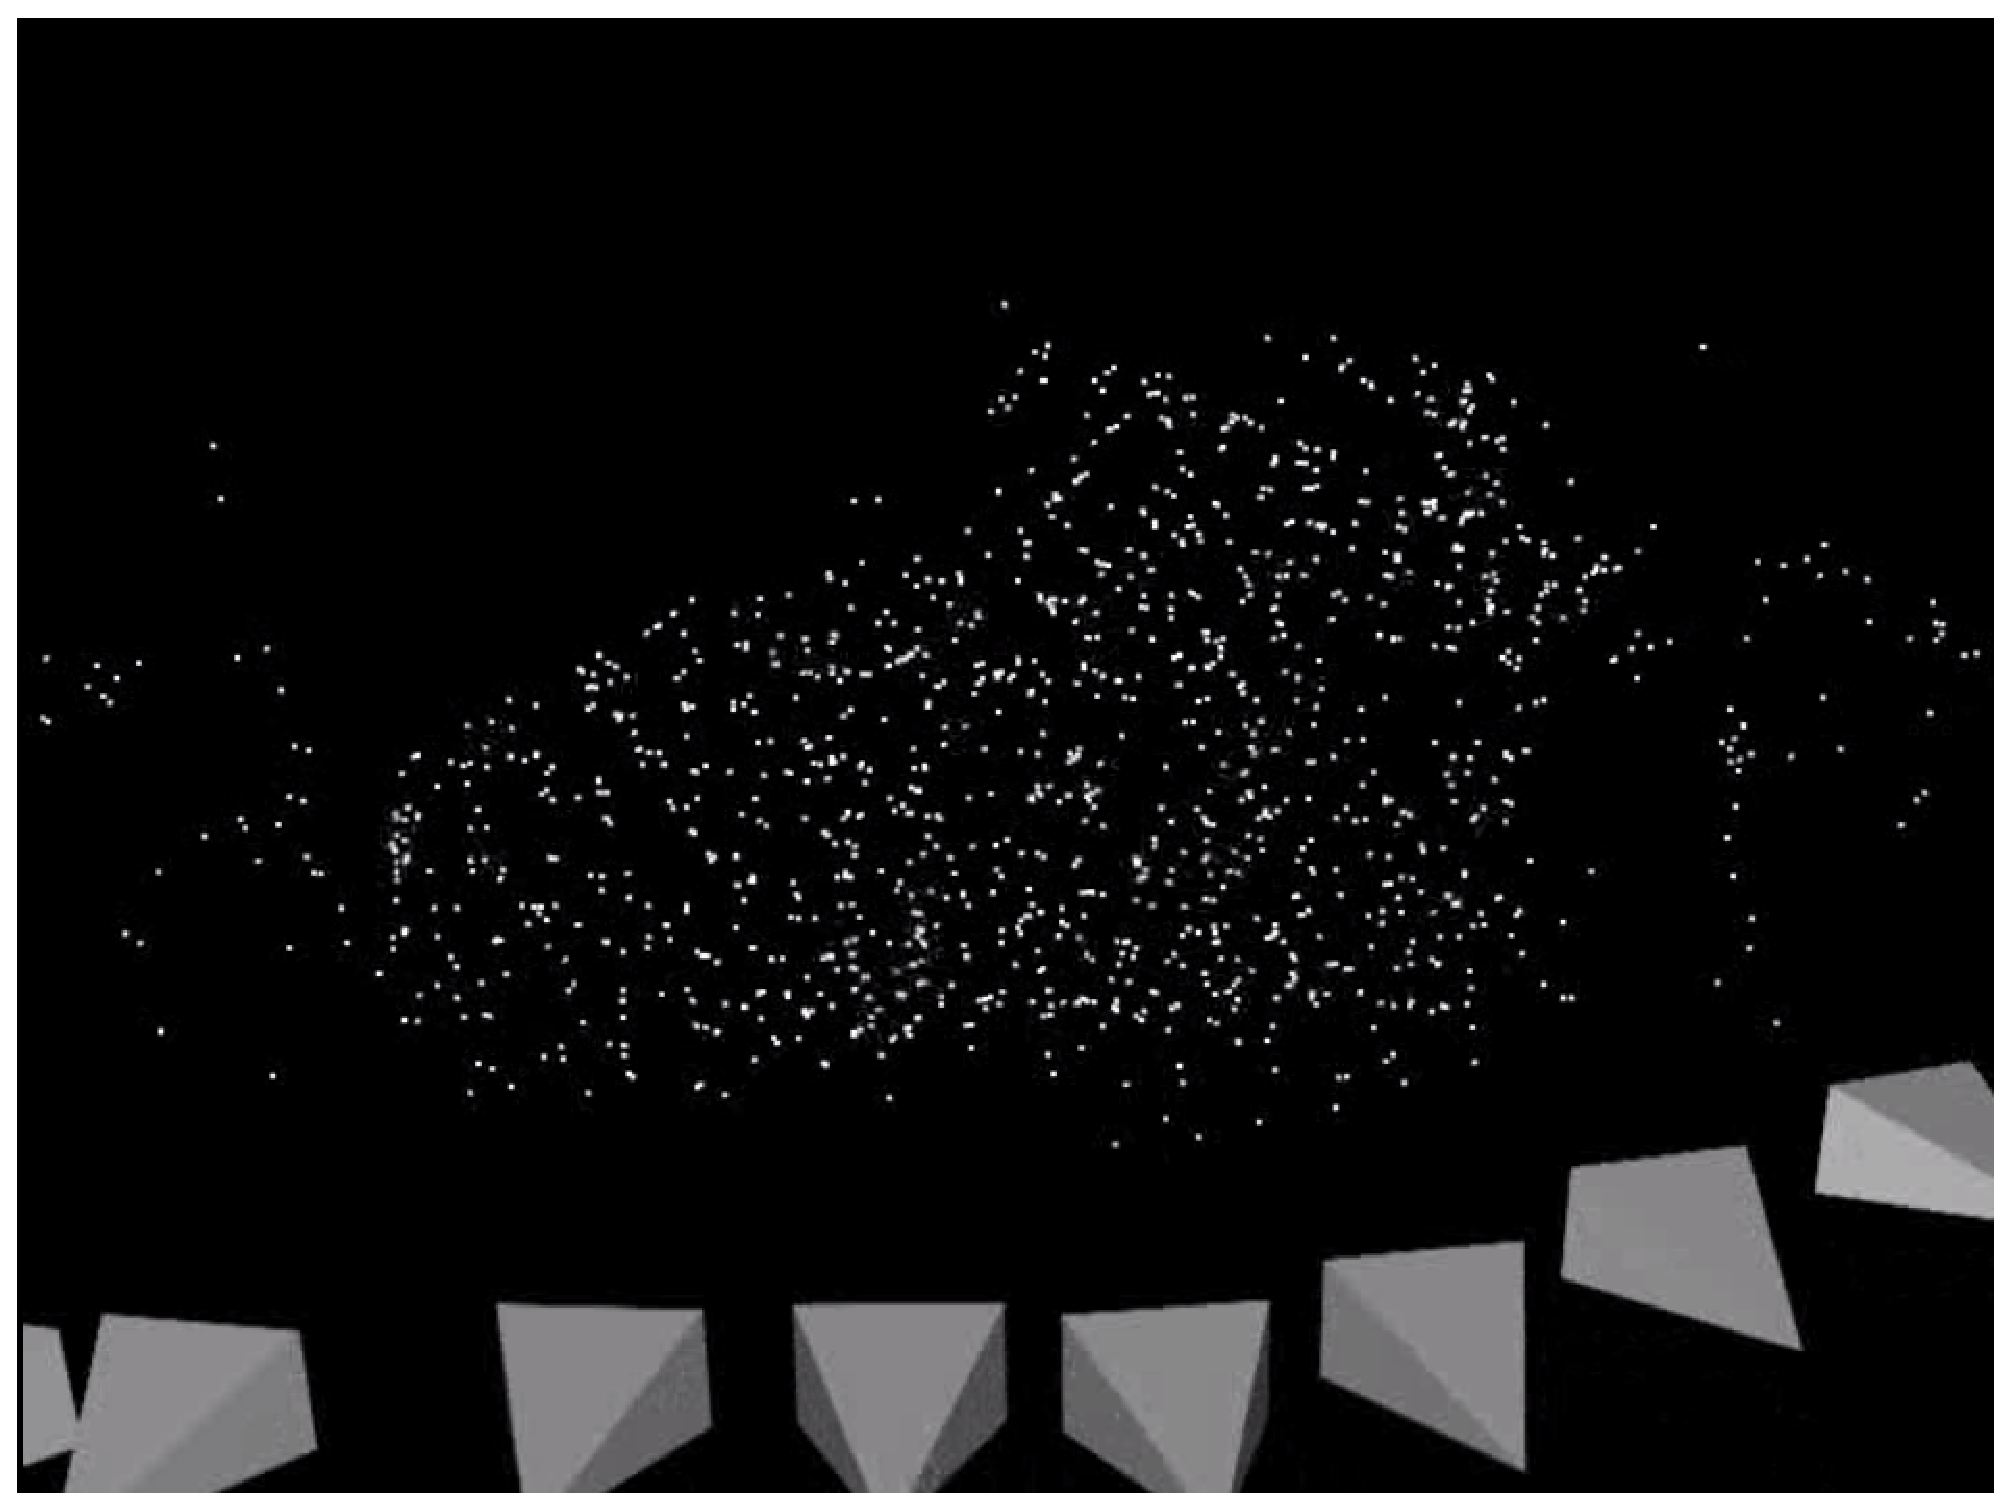
\includegraphics[scale=.2]{nuvem2}}
\\
\subfloat{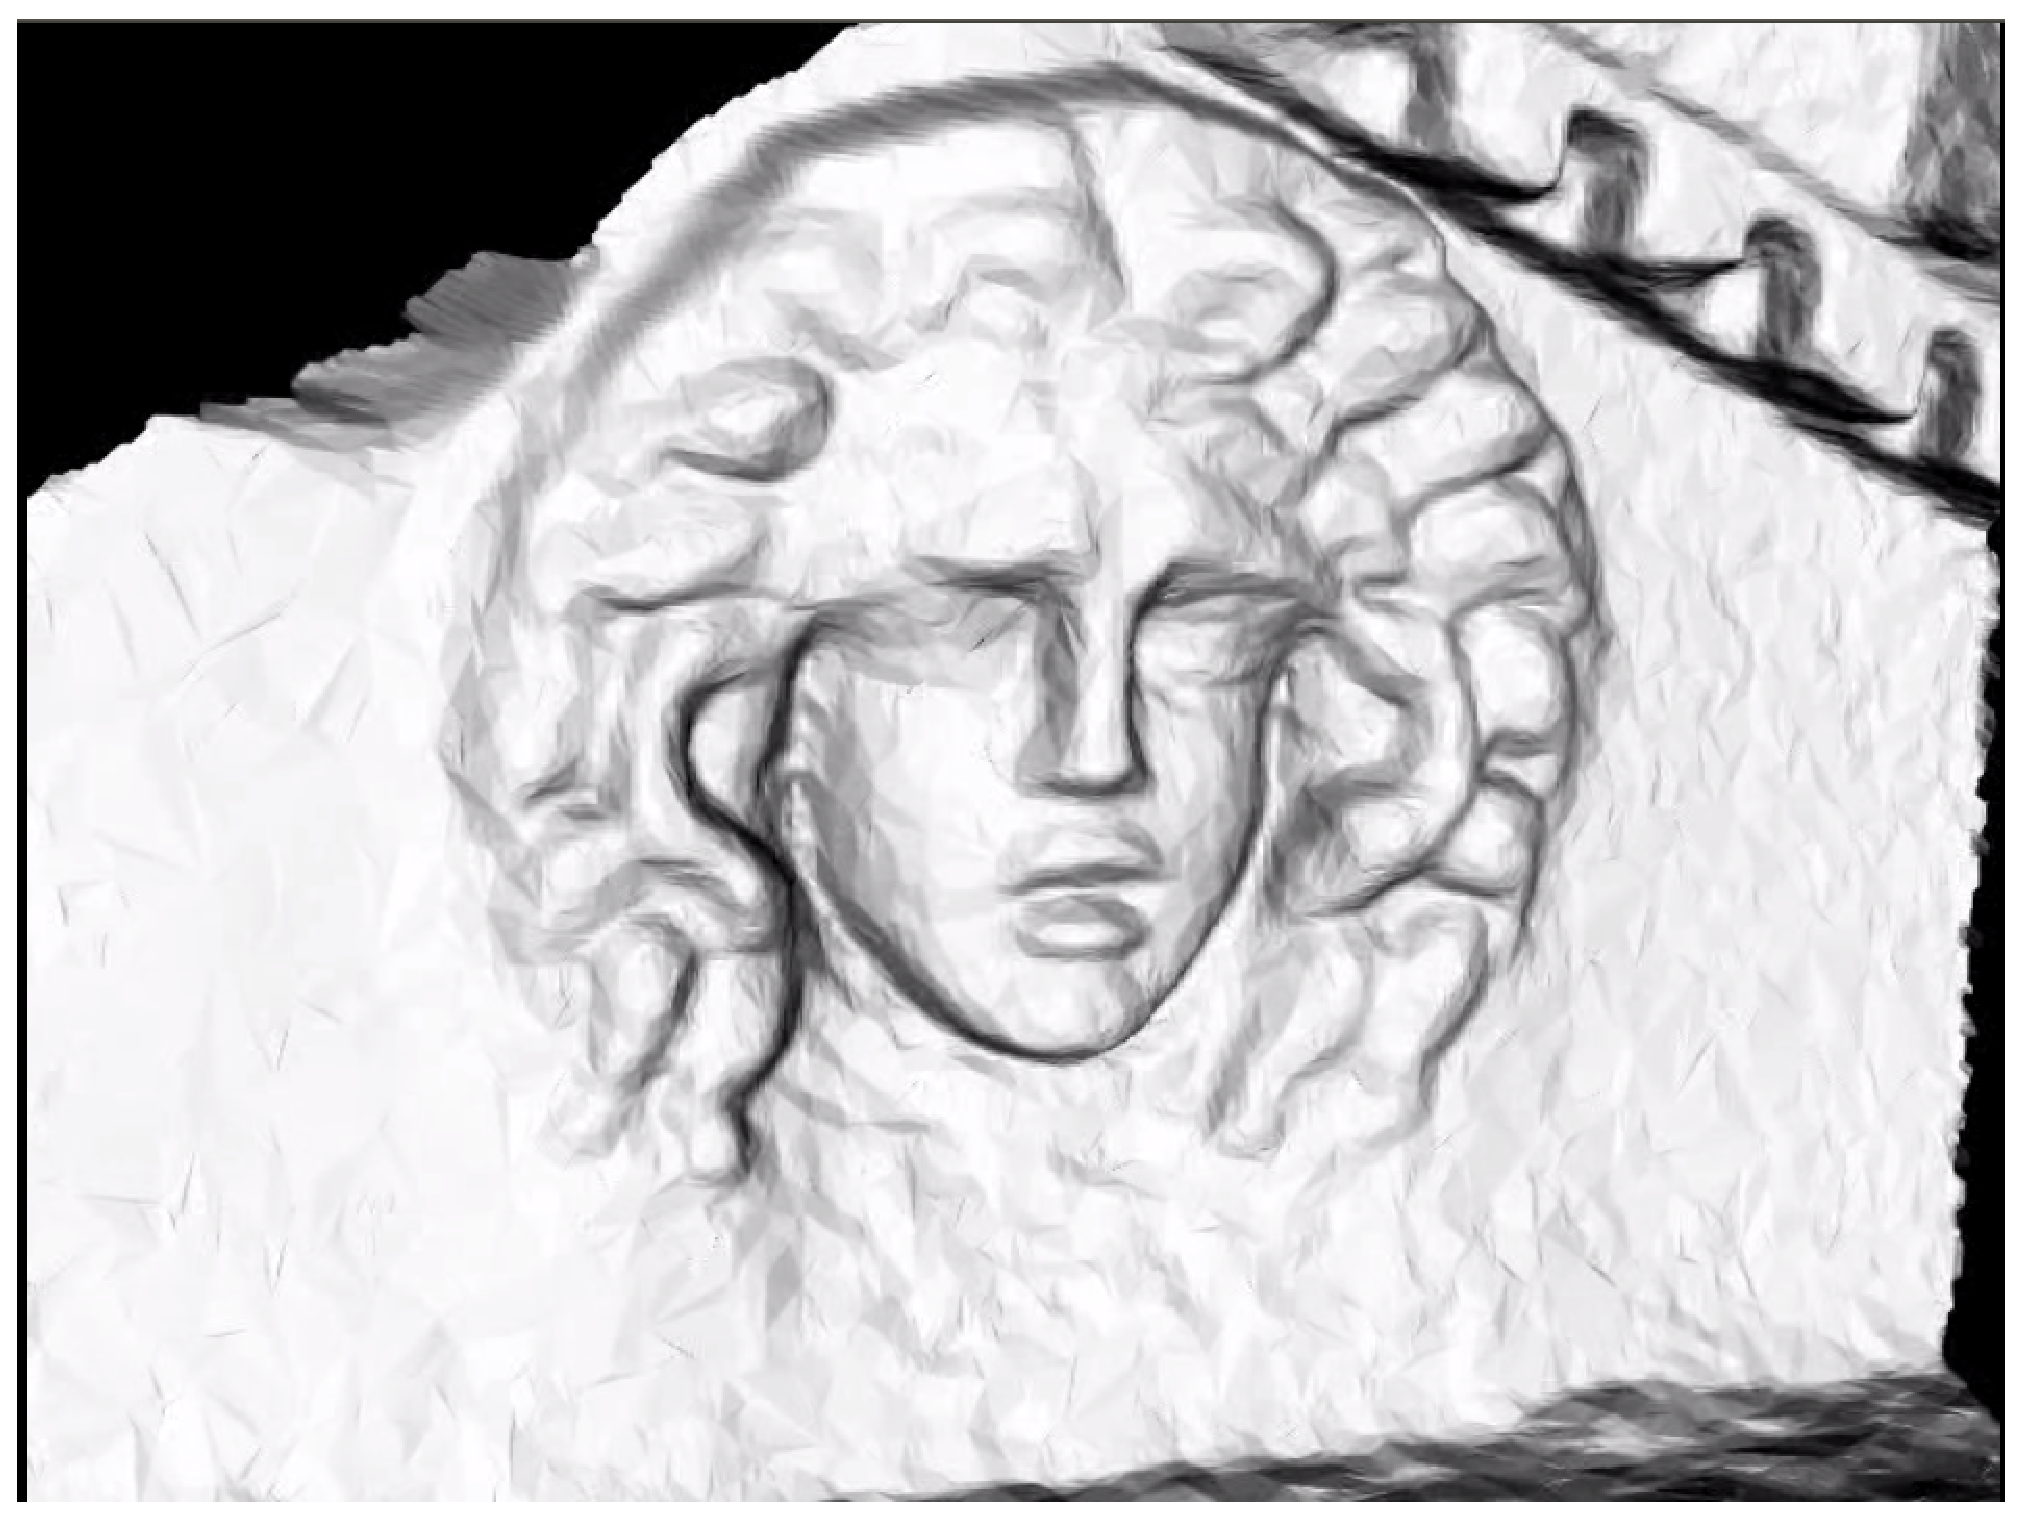
\includegraphics[scale=.2]{texturizacao2}}
\quad
\subfloat{\includegraphics[scale=.2]{texturizacao-realmente}}
\caption{{\it Em cima, duas imagens extraídas de um vídeo (utilizado em reconstrução 3D) da estátua da Meduza. No meio, a nuvem de pontos obtida após a reconstrução 3D juntamente com as posições da câmera. Em baixo, aplicação de interpolação de pontos e texturização.}}
\label{fig.medusa}
\end{figure}

\subsection*{Visão geral e objetivos}

A seção \ref{sec.geo-1-2-cam} engloba a teoria básica de geometria projetiva utilizada em visão computacional 3D, com abordagens em termos de álgebra linear e usando o tipo de notação mais difundido entre pesquisadores da área. Além dos conceitos básicos, também são apresentados alguns conceitos e definições um pouco mais avançados indispensáveis ao entendimento das demais seções da dissertação, tudo com a finalidade de facilitar a compreensão do leitor sem a necessidade de consulta em outras publicações. Em seguida, há a apresentação da geometria epipolar, num sistema de visão estéreo com duas câmeras, bem como extração da matriz fundamental e a reconstrução das câmeras, usando essa abordagem bifocal que é mais comum do que a abordagem trifocal.

Na seção \ref{sec.astrom} temos o detalhamento de um artigo recente e representativo para a reconstrução de uma câmera a partir de objetos geométricos em 3D e suas respectivas imagens em 2D, \citep{bib:kuang}. A importância dessa publicação se verifica na utilização do quatérnion de Hamilton para a parametrização da matriz de rotação da câmera, pois desta forma a matriz que possui nove componentes é parametrizada com apenas três variáveis. Outra vantagem é utilização das Bases de Gr\"obner e da matriz de Ação para solução computacional de sistemas de equações polinomiais de grau elevado e com muitas variáveis.

A geometria trifocal e suas características são abordadas na seção \ref{sec.geo-tri}, juntamente com a descrição dos benefícios do uso dessa geometria num sistema com três câmeras em comparação com uso da geometria epipolar entre cada par de câmeras. Após as comparações são apresentados métodos para a extração das matrizes fundamentais e métodos de reconstrução das câmeras a partir do tensor trifocal.  

Na seção \ref{sec.nister} há o detalhamento matemático da abordagem mais eficiente, até a presente data, para a reconstrução 3D das câmeras num sistema trifocal, \citep{2503343}. O artigo é bastante denso, com 25 teoremas, e apresenta a reconstrução de duas câmeras num sistema bifocal utilizando uma intrincada rede de conhecimentos de geometria projetiva. Depois da reconstrução das duas primeiras câmeras, é utilizada a reconstrução 3D de pontos para a reconstrução da terceira câmera, num procedimento similar ao apresentado na seção \ref{sec.astrom}, ou seja, os dois artigos quase se complementam. Esse trabalho deixa bem clara a dificuldade de se realizar a reconstrução num sistema com três imagens de quatro pontos 3D numa cena.

No apêndice \ref{sec.Apen-A} são fornecidas ferramentas de álgebra linear acompanhadas de algumas definições mais restritas à assimilação da dissertação. No apêndice \ref{sec.geo-algebrica} há uma breve introdução aos conceitos básicos de geometria algébrica seguidos da apresentação (informal e em termos de exemplos) de uma teoria para resolução de sistemas de equações polinomiais com várias variáveis.


\section{Pesquisas Anteriores para a Determinação de Pose}
 
 O problema da determinação da pose de uma câmera  tem sido estudado extensivamente pela comunidade da área de visão computacional. Vamos citar alguns exemplos da determinação da pose de uma câmera.

\subsection{Usando três Pontos}
O caso mínimo da determinação de uma pose usando três pontos foi estudado por \cite{fischler}, e em seus estudos foi relatado o seguinte problema: 

``Dado um grupo de $m$ pontos de referência, cujas coordenadas 3D são conhecidas em um certo sistema de coordenadas, e dada uma imagem de um subconjunto desses $ m $ pontos de referência, determinar a localização (no sistema de coordenadas desses pontos de referência) do ponto onde a imagem foi registrada."

Assume-se que se conhece a correspondência entre os pontos de referência e os respectivos pontos na imagem, são conhecidos o ponto principal e o comprimento da distância focal para facilitar o cálculo dos ângulos entre pontos de referência a partir do centro da câmera, e por fim, assume-se que a câmera está localizada fora e ``acima" da região convexa formada pelos pontos de referência.
Desta forma, calculando as três distância entre o centro da câmera e  três pontos de referência (chamadas de ``pernas"), é possível determinar a posição da câmera bem como a orientação do plano da imagem. Nota-se que esses três pontos de referência formam um triângulo e, juntamente com o  centro da câmera, forma-se um tetraedro. Para calcular essas três ``pernas" pode-se aplicar a lei dos cossenos e formar um sistema com três equações. Em seguida, [10] explicita uma solução algébrica para o sistema bem como uma solução iterativa, calcula o centro da câmera e a orientação do plano da imagem.

Muitas outras formulações para problemas desse tipo foram comparadas e revisadas por \cite{haralick}. 

\subsection{Usando três Linhas}
 Para correspondência usando linha foi encontrada uma solução mínima usando três linhas e suas correspondências por \cite{chen}, como se segue:

Neste artigo não é determinada a pose de uma câmera, mas sim feita uma exposição para detrminação da localização de objetos em geral, com relação a um detrminiado sistema de coordendas. Sendo $\mathbf{m_i} $ a direção de uma linha $\mathbf{L_i} $ e $\mathbf{n_i} $ o vetor unitário normal a um plano $\mathbf{F_i} $. Além disso, $\mathbf{p_i} $ é a posição de um ponto na linha $\mathbf{L_i} $ e $\mathbf{d_i} $ é a distância entre $\mathbf{F_i} $ e a origem do sistema de coordenadas. O problema pode ser matematicamente formulado:
Dados $\mathbf{m_i} $,$\mathbf{n_i} $,$\mathbf{p_i} $,$\mathbf{d_i} $, determinar $ R $ e $ \mathbf{t} $ de maneira que 
\begin{equation*}
{\bf n}_i^{T}\,R\,{\bf m}_i = 0 \qquad {\bf n}_i^T\,(R\,{\bf p}_i+{\bf t}) = {\bf d}_i
\end{equation*}

As equações significam que, para uma matriz de rotação, o vetor linha rotacionado é perpendicular ao vetor normal. E, para um vetor de translação, o ponto transladado perntencerá ao plano. Mais ainda, toda a linha que contém esse ponto estará contida no plano. Como são necessárias seis restrições para a matriz de rotação e o vetor de translação, precisa-se de pelo menos três pares de correspondência para resolver o problema, pois cada par nos fornece duas equações.

A solução dada por \cite{chen} é chamada solução canônica e consiste basicamente em calcular a matriz de rotação usando a primeira relação, definindo essa matriz com uma multiplicação de outras três matriz de rotação, onde cada uma produz uma rotação em torno de um eixo, os quais formam entre si uma base perpendicular. A primeira relação gera um sistema com duas equações onde é dada uma solução numérica. As entradas do vetor de translação são lineares na segunda relação, e são calculadas após o cálculo da matriz de rotação, usando um sistema com três equações.

Outro desenvolvimento envolvendo linhas pode ser encontrado em \cite{dhome}.

\subsection{Usando Combinação de Pontos e Linhas}
Recentemente, um caso mínimo usando combinação de pontos e linhas foi publicado \cite{ramalingam}. Na correspondência entre pontos, usa-se o fato de que os pontos  ${\bf X}$ 3D na cena, ${\bf x}$ 2D na imagem e ${\bf C}$ o centro da câmera, estão alinhados. Esses pontos são empilhados numa matriz $3\times4$, onde cada submatriz $3\times3$ terá determinante zero por conta da linearidade dos pontos. As entradas do ponto 2D imagem nessa matriz são colocadas em função da matriz de rotação $R$ e do vetor de translação ${\bf t}$, retirados da equação de projeção $\lambda\,{\bf x}={\bf P}\,{\bf X}$.

\begin{center}
$\begin{bmatrix}
C_1 & X_1 & R_{1,1}\,X_1\,+\,R_{1,2}\,X_2\,+\,R_{1,3}\,X_3\,+\,t_1 \\ 
C_2 & X_2 & R_{2,1}\,X_1\,+\,R_{2,2}\,X_2\,+\,R_{2,3}\,X_3\,+\,t_2 \\ 
C_3 & X_3 & R_{3,1}\,X_1\,+\,R_{3,2}\,X_2\,+\,R_{3,3}\,X_3\,+\,t_3 \\ 
1 & 1 & 1
\end{bmatrix} $
\end{center}

Apesar do cálculo de quatro derterminantes na matriz acima, temos apenas duas restrições já que nem todas as equações são L.I.

Uma abordagem similar é construída para as correspondências entre linhas. Uma linha na cena possui pontos extremos ${\bf X}_1$ e ${\bf X}_2$, a linha correspondente na imagem possui extremos ${\bf x}_1$ e ${\bf x}_2$. Esses quatro pontos saõ coplanares juntamente com o centro ${\bf C}$ da câmera e, por isso, o determinante da matriz abaixo deve ser zero.

\begin{center}
$\begin{bmatrix}
C_x & X_{1,x} & X_{2,x} & R_{1,1}\,X_{1,x}\,+\,R_{1,2}\,X_{1,y}\,+\,R_{1,3}\,X_{1,z}\,+\,t_1 \\ 
C_y & X_{1,y} & X_{2,y} & R_{2,1}\,X_{2,x}\,+\,R_{2,2}\,X_{2,y}\,+\,R_{2,3}\,X_{2,z}\,+\,t_2 \\ 
C_z & X_{1,z} & X_{2,z} & R_{3,1}\,X_{3,x}\,+\,R_{3,2}\,X_{3,y}\,+\,R_{3,3}\,X_{3,z}\,+\,t_3 \\ 
1 & 1 & 1 & 1
\end{bmatrix} $
\end{center}

O determinante dessa matriz fornece uma restrição usando a imagem ${\bf x}_1$, mas consegue-se outra restrição com o determinante de uma matriz similar usando a imagem ${\bf x}_2$. Assim, combinando duas linhas e um ponto ou dois pontos e uma linha, obtém-se as seis restrições necessárias. Com uma mudança de coordenadas que satisfaz algumas condições, ficam determinados os pontos na imagem, na cena e o centro da câmera. Além disso, o sistema de equações fica reduzido a um polinômino de grau 4 a 8, bem menor que o original (antes da mudança de coordenadas) que era 64. Outro estudo bastante interessante usando combinações de pontos, linhas e tagentes  pode ser encontrado em \cite{bib:kuang}. Nesse estudo, observa-se ainda a aplicação de técnicas recentes de resolução de sistemas de equações polinomiais multivariadas, baseadas em geometria algébrica. 

\subsection{Usando quatro Pontos não Coplanares}
A generalização para casos não planares, o caso mínimo usando quatro pontos 2D-3D foi primeiramente resolvido por \cite{triggs}. A ideia basica é determinar a pose e a distancia focal usando quatro correspondencias e tomando a matriz de calibraçao com os valores padronizados:

\begin{center}
$\begin{array}{cc}
K =  & \begin{bmatrix}
 0 & 0 & 0 \\ 
 0 & 1 & 0 \\ 
 0 & 0 & 1/f
\end{bmatrix} 
\end{array}$
\end{center}

O primeiro passo é parecido com o algoritmo DLT onde dado um ponto 3D e sua imagem $\lambda\,{\bf x} = P\,{\bf X}$, elimina-se a profundidade $\lambda$ com o produto cruzado ${\bf x}\times P\,{\bf X} = {\bf 0}$ e escolhe-se duas restrições em $P$. Transformando ${\bf x}$ numa matriz de \textit{Householder}, as restrições podem ser reunidas numa matriz $2\,n\times 12$, e no caso do uso de quatro pontos teremos uma matriz $8\times 12$ que tem posto $8$ e deixa $4$ espaços nulos. $P$ pode ser descrita como:

\begin{center}
$P = P(\mu)\equiv\sum_{i=1}^d{\mu_i\,P_i} $,
\end{center}

onde $P_i$ são as matrizes $3\times 4$ correspondentes a cada vetor base do espaço nulo, os quais são calculados numericamente através da decomposição SVD.

Sendo a decomposição $P\simeq K\,R(I| -{\bf t})$, a matriz quádrica absoluta e sua imagem

\begin{center}$
\begin{array}{cc}
\begin{array}{cc}
\Omega \equiv  & \begin{bmatrix}
1 & 0 & 0 & 0 \\ 
0 & 1 & 0 & 0 \\ 
0 & 0 & 1 & 0 \\ 
0 & 0 & 0 & 0
\end{bmatrix} 
\end{array} 
 & \text{e} \quad \omega \equiv P\,\Omega P^{T} \simeq KK^{T} \text{, respectivamente.}
\end{array}$ 
\end{center}

Assim pode-se converter as restrições em $K$ naquelas das candidatas $P(\mu)$ ou nas imagens $\omega$:

\begin{center}
$\omega  = \omega (\mu) \equiv P(\mu)\,\Omega P(\mu)^T$
\end{center}  

Como $K = diag((f,f,1)$ então $K\,K^T = diag(f^2,f^2,1)$ e, consequentemente, 
\begin{center}
$\omega _{1,1} = \omega_{2,2}$ \quad e \quad $\omega_{1,2} = \omega_{1,3} = \omega_{2,3} = 0$
\end{center}

Assim temos um sistema de equações quadráticas nas quatro variáveis $\mu_i$ que tem pelo menos uma solução. Pode-se usar a decomposição SVD para obter os $\mu_i$, sustituí-los em $P(\mu)$ para obter $P$, em seguida fazer a decomposição de $P$ para obter pose e calibração. A matriz resultante é grande, $80\times 56$ mas ainda sim é tratável.


 Outros autores como \cite{bujnak} resoveram para um caso mínimo de quatro pontos para câmeras sem conheciemnto da distância focal e distorção radial.

\subsection{Usando Pontos-Tangentes}
Em \cite{Fabbri:Giblin:Kimia:ECCV12} uma solução é dada usando um problema mínimo de dois pontos-tangentes,$\lbrace ({\bf X}_1^w,{\bf T}_1^w),({\bf X}_2^w,{\bf T}_2^w)\rbrace$, e suas respectivas imagens $\lbrace ({\bf x}_1,{\bf t}_1),({\bf x}_2,{\bf t}_2)\rbrace$. No artigo é demonstrado que a solução pode ser obtida resolvendo um sistema com duas equações:

\begin{center}
$\begin{cases}
{\bf x}_1^T\,{\bf x}_1\,\rho_1^2 - 2\,{\bf x}_1^T\,{\bf x}_2\,\rho_1\,\rho_2 + {\bf x}_2^T\,{\bf x}_2\,\rho_2^2 = ||{\bf X}_1^w - {\bf X}_2^w||\\
Q(\rho_1,\rho_2) = 0,
\end{cases}$
\end{center}

onde $\rho$ é a profundidade em ${\bf x} = \rho\,{\bf X}$, $Q$ é um polinômio de grau 8, e a pose da câmera $R, {\bf \tau}$ relativa ao sistema de coordenadas do mundo é definida por ${\bf X} = R\,{\bf X}^w  + \tau$. 

Fazendo-se umas substituições e isolando $R\, \text{e}\, \tau$ temos:

\begin{center}
$\begin{cases}
R = [({\bf X}_1^w - {\bf X}_2^w)\,{\bf T}_1^w\,{\bf T}_2^w]^{-1} \cdot [\rho_1\,{\bf x}_1 - \rho_2\,{\bf x}_2\,\rho_1\,\frac{g_1}{G_1}\,{\bf t}_1 + \frac{\rho_1'}{G_1}\,{\bf x}_1\,\rho_2\,\frac{g_2}{G_2}\,{\bf t}_2 + \frac{\rho_2'}{G_2}\,{\bf x_2}]\\
\tau = \rho_1\,{\bf x}_1 - R\,{\bf X}_1^w.
\end{cases}$
\end{center}

Em material suplementar estão disponíveis expressões para $\frac{g_1}{G_1}, \frac{g_2}{G_2}\text{(razão das velocidades)}, \rho_1 \,\text{e}\, \rho_2$. 

\texttt{ correspondência necessária é reduzida a uma única correspondência local feita por [20 - koser,koch].Contudo, esta última configuração é muito sensível aos ruídos medidos na correspondência. Para determinação de pose de câmera sem conhecimento da distância focal, o caso com imagens no mesmo plano foi formulado por [1 - abidi,chandra].  Soluções eficientes  e numericamente estáveis foram desenvolvidas por [4 - bujnak et.al.]. Combinando correspondências 2D-2D e 2D-3D, [19 - josephson, astrom, et. al.] investigaram muitos casos mínimos para determinação da pose sem conhecimento da distância focal.   }


\section{Geometria de Uma e Duas Câmeras}

\subsection{Notação Básica de Geometria Projetiva}

Nesta seção, faremos uma breve introdução aos conceitos básicos de Geometria Projetiva e usaremos a notação contida em (citar hartley), por ser o tipo de notação mais difundido entre pesquisas de visão computacional. Para uma abordagem mais profunda do assunto o leitor pode pesquisar o referido autor.  

\subsubsection{O Espaço Projetivo em Duas Dimensões}



$\Longrightarrow$ A Reta


Sabemos que uma reta no plano $\mathbb{R}^{2}$ pode ser representada pela equação $a\,x+b\,y+c=0$, onde a reta fica perfeitamente determinada pelos valores das constantes $a,b,c$. Desta forma, podemos representar retas através de vetores, e assim a reta $a\,x+b\,y+c=0$ seria representada por $(a,b,c)^T \in \mathbb{R}^{3}$, utlizando o símbolo em negrito $\lightrgb$ para indicar tal vetor escrito em coluna, por padrão. Portanto $\lightrgb = (a,b,c)^T$. Note que a relação entre uma dada reta e o seu respectivo vetor não é biunívoca, pois o vetor $k\,(a,b,c)^T$, tal que $k \in \mathbb{R}$, representa a reta $k\,a\,x+k\,b\,y+k\,c=0$ que é a mesma reta $a\,x+b\,y+c=0$. Temos, então, infinitos vetores (chamados paralelos na Álgebra Linear) que representam uma mesma reta e formam uma classe de equivalência, onde essa classe pode ser repsentada por qualquer um de seus vetores. Os vetores de uma classe de equivalência, definida pela multiplicação por um escalar, são conhecidos como vetores {\it homogêneos}. O conjunto de classes de equivalência de vetores em $\mathbb{R}^{3} - (0,0,0)^T$ forma o {\it Espaço Projetivo} $\mathbb{P}^{2}$. O vetor $(0,0,0)^T$ foi excluído por não representar reta alguma. Após essas considerações, dizemos que uma reta no plano é representada pelo vetor $(a,b,c)^T$ em {\it coordenadas homogêneas}.
\\

$\Longrightarrow$ O Ponto


Sabemos também, que em $\mathbb{R}^{2}$ os pontos são representados através de pares ordenados do tipo $(x,y)$, assim cada ponto pode ser identificado como um vetor $(x,y)^T$. Os vetores que se referem a pontos serão representados pelo símbolo em negrito $\x$, que sempre indicará um vetor coluna. Desse jeito, $\x=(x,y)^T$. Sabemos também que um ponto $(x,y)^T$ pertence a uma reta $(a,b,c)^T$ se, e somente se $a\,x+b\,y+c=0$, e podemos realizar essa verificação utilizando multiplicação matricial, escrevendo $\x$ com uma terceira coordenada igual a 1:

\begin{center}
$\begin{array}{ccccc}
 (x,y,1)^T 
&\begin{pmatrix}
 a  \\ 
 b  \\ 
 c 
 \end{pmatrix} 
& = 0 \qquad 
& \text{ou} 
& \qquad \x ^T\lightrgb = 0.
\end{array}$
\end{center}

Ou seja, temos um ponto de $\mathbb{R}^{2}$ representado como um vetor com três coordenadas. Observe que para $k \in \mathbb{R} - \{0\}$, temos:

\begin{center}
$\begin{array}{ccccccc}
 (k\,x,k\,y,k)^T 
&\begin{pmatrix}
 a  \\ 
 b  \\ 
 c 
 \end{pmatrix} 
& = 0
& \qquad \leftrightarrow \qquad
& (x,y,1)^T
&\begin{pmatrix}
 a  \\ 
 b  \\ 
 c 
 \end{pmatrix} 
& = 0.
\end{array}$
\end{center}

Portanto,  variando $k$, podemos considerar os vetores em coordenadas homogeneas $(k\,x,k\,y,k)^T \in \mathbb{P}^2$, como representantes do mesmo ponto $(x,y)^T \in \mathbb{R}^2$, e podemos resgatar nossa representaçao original aplicando o procedimento $(x/k,y/k)^T$, pois $k \ne 0$.

\begin{figure}[!htb]
\centering
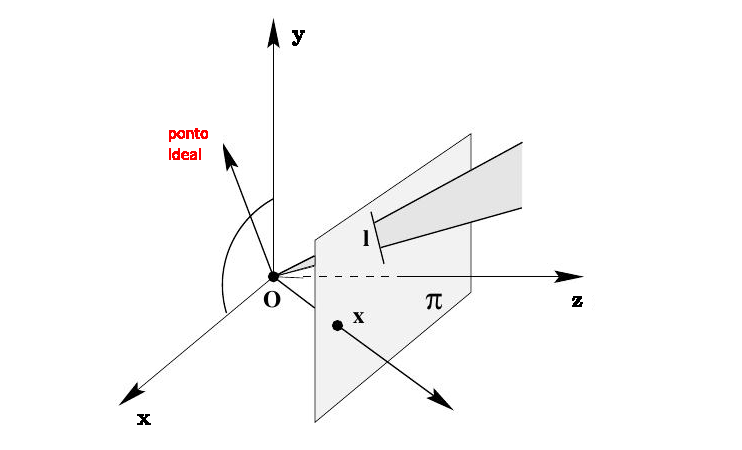
\includegraphics[scale=0.8]{espaco_P2}
\caption{O plano $\pi$ representa o espaço projetivo $\mathbb{P}^2$. Pontos e retas pertencentes a esse espaço são representados, respectivamente, por raios e planos que passam pela origem do $\mathbb{R}^3$.}
\label{plano_P2}
\end{figure}

Podemos pensar no esapaço projetivo como um conjunto de raios passando pela origem do $\mathbb{R}^3$, onde cada raio representa um único ponto, que é a interseção desse raio com o plano $\mathbb{P}^2$. Desta mesma forma, retas em $\mathbb{P}^2$ são formadas por planos. Na figura \ref{plano_P2}, podemos observar com a interseção do raio com o plano define um ponto, assim como a interseção de dois planos definem uma reta.
\\

$\Longrightarrow$ A Cônica


Em geometria Euclidiana, as cônicas são de três tipos principais: elipse, hipérbole e parábola. São definidas, algebricamente, por uma equação do segundo grau em duas variáveis, considerando coordenadas não homogêneas:

\begin{equation*}
a\,x^2+b\,x\,y+c\,y^2+d\,x+e\,y+f=0.
\end{equation*}

Sabemos que um ponto pertence à cônica se ele é solução da equação acima, a qual pode ser representada utilizando multiplicação matricial e vetores em coordenadas homogêneas, com a terceira coordenada configurada como 1:

\begin{center}
$
\begin{array}{cccc}
  (x,y,1)^T 
& \begin{bmatrix}
a & b/2 & d/2\\
b/2 & c & e/2\\
d/2 & e/2 & f
\end{bmatrix}
& \begin{pmatrix}
x\\
y\\
1
\end{pmatrix}
& = 0.
\end{array}
$
\end{center}

Podemos generalizar essas coordenadas homogêneas fazendo as substituições $x = x_{1}/x_{3}$ e $y = x_{2}/x_{3}$, e nossa equação do elípse fica:

\begin{equation*}
a\,x_1^2+b\,x_1\,x_2+c\,x_2^2+d\,x_1\,x_3+e\,x_2\,x_3+f\,x_3^2=0.
\end{equation*}

Novamente em notação matricial:

\begin{center}
$
\begin{array}{cccccc}
  (x_1,x_2,x_3)^T 
& \begin{bmatrix}
  a & b/2 & d/2\\
  b/2 & c & e/2\\
  d/2 & e/2 & f
  \end{bmatrix}
& \begin{pmatrix}
  x_1\\
  x_2\\
  x_3
  \end{pmatrix}
& = 0
& \qquad \text{ou} \qquad
& \x^T\,C\,\x = 0.
\end{array}
$
\end{center}

Já que um ponto pertence à cônica se, e somente se, satisfaz a última equação, temos que $C$ fica definida como a matriz que representa uma cônica no espaço projetivo $\mathbb{P}^2$.

\begin{center}
$
\begin{array}{cc}
C = & \begin{bmatrix}
      a & b/2 & d/2\\
      b/2 & c & e/2\\
      d/2 & e/2 & f
      \end{bmatrix}.
\end{array}
$
\end{center}




\subsubsection{O Espaço Projetivo em Três Dimensões}


$\Longrightarrow$ O Ponto


Analogamente à representação de um ponto no espaço $\mathbb{P}^2$, um ponto no espaço $\mathbb{P}^3$ é repesentado através de coordenadas homogêneas, acrescentando-se uma quarta coordenada ao vetor que representa esse ponto. Desta forma, $\X = (X_1,X_2,X_3,X_4)^T$ e $X_4 \ne 0$, onde $\X$ é a representação em coordenadas homogêneas do ponto $(X,Y,Z)^T \in \mathbb{R}^3$. Para realizar essa mudança basta tomar 

\begin{equation*}
X=X_1/X_4 \,\, ,\, Y=X_2/X_4 \,\,\, \text{e} \,\,\, Z=X_3/X_4.
\end{equation*}


$\Longrightarrow$ O Plano

Temos que a representação algébrica de um plano $\bpi$ no espaço $\mathbb{R}^3$ é dada pela equação

\begin{equation*}
\pi_1\,X+\pi_2\,Y+\pi_3\,Z+\pi_4=0.
\end{equation*}


\subsection{Notação Usada por Fabbri}
Usar figura do artigo.

\subsection{Resumo dos Resultados Fabbri}
Projeção e reconstrução 3D com o uso de tangentes.

\section{Geometria Trifocal}

\subsection{O Problema}

\subsection{Abordagem por Tensor Trifocal}

\subsection{Abordagem do Nistér}
\section{Geometria Diferencial Trifocal}\label{sec:geo:dif:tri}

\subsection{Abordagem do Fabbri}
Problema 2.

\subsection{Nova Solução}

\subsection{Novo Algoritmo}

\subsection{Experimentos com novo Algoritmo}



\section{Aplicações da Geometria Diferencial Trifocal}
(Objetivo: apanhado geral do uso de geometria trifocal e ideias novas)

\subsection{Aplicações em Sistemas de SfM}
Aplicações em structure for motion.

Explicar como utilizar os resultados dos dois últimos capítulos em sistema real.

\subsection{Outras Aplicações}
\input{expe_conc}
\section{Conclusões}

Existe toda uma engenhosidade no emprego de coordenadas homogêneas para fazer com que uma transformação projetiva funcione como uma transformação linear, mesmo que exista (disfarçadamente) a aplicação de uma translação. Além disso, a representação de pontos em coordenadas homogêneas favorece a representação de objetos algébricos abstratos, como pontos no infinito e a cônica absoluta, e a dedução de propriedades não existentes em outras geometrias, como a interseção de retas paralelas.

As pesquisas em visão computacional são auxiliadas por outras áreas da matemática aparentemente desconexas da geometria projetiva, pois na seção \ref{sec.astrom} verificamos a utilização do Quatérnion de Hamilton para parametrizar uma matriz de rotação e das Bases de Gr\"obner e Matriz de Ação na solução de sistemas de equações polinomiais, ambos empregados na determinação de uma câmera $P$. A própria utilização de sistemas de equações polinomiais com muitas variáveis na modelagem de problemas atuais pode se constituir uma novidade para vários pesquisadores.

Constatamos na seção \ref{sec.geo-tri} alguns benefícios do uso do tensor trifocal num sistema com três imagens em detrimento do uso puramente da geometria epipolar. Há a diminuição de alguns casos de degeneração para a correspondência de pontos em três imagens, e há também o benefício da determinação direta de uma reta numa imagem dadas as retas correspondentes nas outras duas imagens. Não há equação para a transferência direta de retas usando apenas geometria epipolar.

O estudo da geometria trifocal envolve uma quantidade grande de conhecimento da teoria básica de geometria projetiva conforme vimos na seção \ref{sec.nister}. Mais ainda, estudar geometria trifocal em problemas de reconstrução requer o conhecimento também da geometria epipolar, não somente em termos de comparação sobre qual das abordagens funciona melhor para reconstrução, mas também para entendermos de que forma a geometria epipolar pode ser útil num sistema com três imagens. Ficou clara a complexidade da tarefa de se determinar as três câmeras num sistema trifocal, e fazer essa determinação em termos de geometria diferencial é uma das fronteiras em visão computacional. 


\nocite{Fabbri:Kimia:CVPR10,Hartley2004,Faugeras,Schmid00,2503343,HartleyLi,koser,kukelova,pajdla,byrod}


\appendix
\section{Possiveis Publicacoes}
\subsection{Trifocal Relative Pose using First-Order Differential Geometry}
Paper mais importante onde resolveriamos o problema para pontos e tangentes.

Capitulos de tese: \ref{sec:geo:dif:tri}

\subsection{Using Trifocal Geometry in Structure from Motion}
Outros titulos:
"Trifocal geometry: Theory and practice in real SfM systems"
"Exploiting Trifocal geometry for bootstrapping SfM systems"
"A Survey of Trifocal Geometry in Structure from Motion"

Capitulos de tese: \ref{sec:apli:geo:dif:tri}

Este responderia às seguintes perguntas:
Qual a vantagem de se iniciar um sistema de autocalibracao externa de cameras usando
geometria trifocal?  O que se ganha em reconstrucao/estereo?

Experimentos:
- implementar bundler com geometria trifocal e observar melhorias
	
\bibliographystyle{plainnat} 
\bibliography{biblio}
\end{document}
